\begin{center}
    \begin{figure}[H]
        \centering

        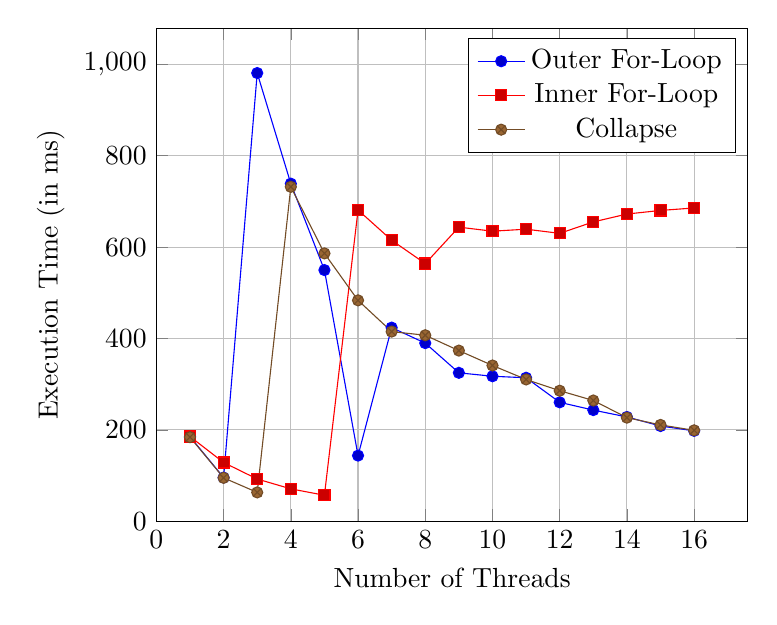
\begin{tikzpicture}
            \begin{axis}[
                title={},
                width=0.75\textwidth,
                xlabel={Number of Threads},
                ylabel={Execution Time (in ms)},
                xmin=0,
                ymin=0,
                grid=major
            ]
                \addplot coordinates {
                    (1,185.148)(2,95.6881)(3,980.967)(4,738.939)(5,549.777)(6,143.797)(7,423.852)(8,389.944)(9,324.914)(10,317.433)(11,314.095)(12,260.368)(13,243.347)(14,228.335)(15,208.511)(16,197.935)
                };
                \addlegendentry{Outer For-Loop}

                \addplot coordinates {
                    (1,185.458)(2,128.647)(3,92.5102)(4,70.9916)(5,57.0061)(6,681.182)(7,615.115)(8,564.001)(9,643.746)(10,634.852)(11,639.269)(12,630.145)(13,655.192)(14,672.427)(15,680.293)(16,685.732)
                };
                \addlegendentry{Inner For-Loop}       

                \addplot coordinates {
                    (1,184.104)(2,95.1303)(3,63.2167)(4,731.922)(5,586.31)(6,483.515)(7,415.139)(8,407.176)(9,373.57)(10,340.994)(11,310.393)(12,285.77)(13,264.366)(14,226.837)(15,210.921)(16,199.055)
                };
                \addlegendentry{Collapse}
            \end{axis}
        \end{tikzpicture}
        \caption{HSV Performance Tests dice\_large.png}
    \end{figure}
\end{center}